% Created 2021-09-12 Sun 22:48
% Intended LaTeX compiler: xelatex
\documentclass[letterpaper]{article}
\usepackage{graphicx}
\usepackage{grffile}
\usepackage{longtable}
\usepackage{wrapfig}
\usepackage{rotating}
\usepackage[normalem]{ulem}
\usepackage{amsmath}
\usepackage{textcomp}
\usepackage{amssymb}
\usepackage{capt-of}
\usepackage{hyperref}
\usepackage[margin=1in]{geometry}
\usepackage{fontspec}
\usepackage{indentfirst}
\setmainfont[ItalicFont = LiberationSans-Italic, BoldFont = LiberationSans-Bold, BoldItalicFont = LiberationSans-BoldItalic]{LiberationSans}
\newfontfamily\NHLight[ItalicFont = LiberationSansNarrow-Italic, BoldFont       = LiberationSansNarrow-Bold, BoldItalicFont = LiberationSansNarrow-BoldItalic]{LiberationSansNarrow}
\newcommand\textrmlf[1]{{\NHLight#1}}
\newcommand\textitlf[1]{{\NHLight\itshape#1}}
\let\textbflf\textrm
\newcommand\textulf[1]{{\NHLight\bfseries#1}}
\newcommand\textuitlf[1]{{\NHLight\bfseries\itshape#1}}
\usepackage{fancyhdr}
\pagestyle{fancy}
\usepackage{titlesec}
\usepackage{titling}
\makeatletter
\lhead{\textbf{\@title}}
\makeatother
\rhead{\textrmlf{Compiled} \today}
\lfoot{\theauthor\ \textbullet \ \textbf{2021-2022}}
\cfoot{}
\rfoot{\textrmlf{Page} \thepage}
\titleformat{\section} {\Large} {\textrmlf{\thesection} {|}} {0.3em} {\textbf}
\titleformat{\subsection} {\large} {\textrmlf{\thesubsection} {|}} {0.2em} {\textbf}
\titleformat{\subsubsection} {\large} {\textrmlf{\thesubsubsection} {|}} {0.1em} {\textbf}
\setlength{\parskip}{0.45em}
\renewcommand\maketitle{}
\author{Houjun Liu}
\date{\today}
\title{Mason Ch 1 and 2}
\hypersetup{
 pdfauthor={Houjun Liu},
 pdftitle={Mason Ch 1 and 2},
 pdfkeywords={},
 pdfsubject={},
 pdfcreator={Emacs 28.0.50 (Org mode 9.4.4)}, 
 pdflang={English}}
\begin{document}

\maketitle


\section{Mason Ch.1 + 2}
\label{sec:org8eebc61}
\begin{html}
<!--
\begin{itemize}
\item European nations began to make international alliances
\item Shifted power to prevent any one country from becoming too powerful
\item Whole economic system begins to be challenged by the end of the 18th century, when \href{KBhHIST201TheEnlightenment.org}{KBhHIST201TheEnlightenment} happened, followed by French Revolution, Industrial Revolution, and solidification of the middle class
\item \href{KBhHIST201Enlightenment.org}{KBhHIST201Enlightenment}
\end{itemize}
-->
\end{html}

\begin{itemize}
\item Applied methods of scientific revolution to study of society
\item Believed natural laws governed human behavior + human institutions
\item John Locke

\begin{itemize}
\item Got on the notion that reason was derived from experience
\item Human nature is essentially good, and character is shaped by
education and upbringing
\item Hence, good societies w/ good education will create a better society
\item Man process natural + inalienable rights to life, liberty, and\ldots{}
property?
\item Political communities are formed by popular consent
\item Had huge influence across the Atlantic
\end{itemize}

\item Jean-Jaques Rousseau

\begin{itemize}
\item "Man is born free, and everywhere he is shackled"
\item Believes that society corrupts and distorts man's natural freedom
and equality
\item Negotiated by social contract
\end{itemize}

\item Adam Smith

\begin{itemize}
\item Applied Enlightenment ideas to economy and market
\item Argued that government inference in the economy violated natural
forces of competition, supply, and demand
\item Self-interest could work for the common good
\item Individual greed + private accumulation of wealth => free market
forces are at play
\item Argued for system of \emph{laissez-faire} => daoistic management of
economy
\item CLAIM: Ideas ultimately influence the development of capitalism
\end{itemize}

\item Perhaps one of the causes of the French Revolution
\item Ideas raised by Enlignment => profoundly setting the direction of
social order
\item Attacked basis of \emph{acien régime}
\item Enlightment Influence
\item Introduced governmental reforms
\item Created new ideas on goverment: \textbf{liberalism}, \textbf{socialism},
\textbf{communism.}
\item French Revolution => 1789
\item Although year for the declaration of the Rights of Man, 1789 is
overshodowed by a whole timeline

\begin{itemize}
\item 1792 => Louis XVI dethroned
\item 1793 => Louis XVI executed
\item 1799 => Napoleon
\item 1815 => Monarchy is back
\end{itemize}

\item During the revolutionary period, France perhaps was the most
significant country

\begin{itemize}
\item Louis XIV established France as centre of power

\begin{itemize}
\item Most populous
\item Leading in arts and sciences
\item Leading in philosophical thought a la Enlightenment
\end{itemize}

\item Cause of revolution

\begin{itemize}
\item Long term

\begin{itemize}
\item Socioeconomic change of the 18th century
\item The Freaking Enlightment
\item Weakening monarchy\\
\end{itemize}

\item Short term

\begin{itemize}
\item Inefficient tax system got the country stripped of money
\item France also dumped a lot of money on Amercias
\item Created economic depression

\begin{itemize}
\item 1726-1789 => cost of living +62\%, wages only +25\%
\item British textile caused massive unempolyment
\item 1788 brought with it famine
\item Louis XVI himself is also quite weak
\end{itemize}
\end{itemize}

\item The Revolution

\begin{itemize}
\item Third estate (peseant) general decided to go rougue (to a tennis
court) when called by the King to discuss tax plans and come up
with their own National Assembly

\begin{itemize}
\item "Whenever we meet, there is the nation."
\item The King, noticing this, took the army to quell the third
estate generals
\item Millitias began forming throughout the city
\item July 14th, 80,000 people stored Bastille prision + seized the
governor of the fortress. This became \textbf{Bastille day}, a French
holiday!
\item With this example, peseants began raiding their landlords
\end{itemize}

\item The suddenly official National Assembly abolished lordish feutal
payments + freed the peseants
\item Tennis Court Oath => Won't stop until new revolution
\item August 16th, the Dec. of the Rights of Man was published => the
French Dec. of Indp.
\item Reflects Enlightenment Ideals => "natural, inalienable, and
sacred rights of man\ldots{} Liberty, property, security, and
resistance to oppression"
\item 6000 woman\ldots{} just decided to chuck the King back into Paris.
\#how???
\item Then, the National Assembly just pretended that they ran the
nation

\begin{itemize}
\item Using monarch as de jurie figurehead
\item Seized all Church property
\item Required clergy election to be public, forced the clergy to be
loyal to the nation
\item New constitution was presented => elected legislative assembly
w/ king only the power as suspensive veto
\end{itemize}
\end{itemize}

\item Louis XVI fled Paris and appealed to all other monarchs => Russian
empress declared "affairs of France were the concern of all
crowned heads."
\item Prussia and Austria began to try to invade France working with the
French king; however, 1792, another insurrection quelled them.
\item The National Convention scratched the monarchy part out of the
constitution, and that was that.
\end{itemize}
\end{itemize}

\item Then, "normal" politics happened

\begin{itemize}
\item The Manhood sufferange movement 1789 => 1971, at which point it's
abandoned
\item Georges Danton + Max Robespirre jockied for power
\item Clubs and meetings established
\item Section assemblies drew many commoners into political activity
\item Then, by a narrow vote, Louis was convicted and confirmed to be
executed
\end{itemize}

\item Then, everyone piled on:

\begin{itemize}
\item Britain Holland, Spain, Austria, Prussia formed a coalition against
France
\item the Convention established a Public Safety committee

\begin{itemize}
\item Created a period called The Terror => putting on trial and killing
everyone who opposed the revolution
\item 40,000 died under this system
\item And so did the leaders of the Terror Danton and Robespierre
\end{itemize}

\item After the Terror, the Convention decided the current constitution
was not good enough --- scrapping it and writing another one after
establishing a five-man Directory for executive power
\item The Directory later became illegitamate, causing, you guessed it, a
\emph{coup d'état} that, you did'nt guess it, established the Monarchy
again!
\end{itemize}

\item Napoleon and the \emph{coup d'état}
\item General in 1793
\item Put down a loyalist uprising in 1795, making him famous
\item Crushed the Austrian forces while he is at it, making him famous
\item Elected cosul in 1802, and just crowned himself in 1804
\item Napoleon acted as the one-man-Directory --- creating a system similar
to true Constitutional Monarchy

\begin{itemize}
\item Weakened representative institutions
\item Censored the press
\item Put down rebellions
\item Did the Terror, but to both royalists and true republicans
\item Made peace with the Catholic Church
\item Introduced new legal code that is still in French law today\\
\end{itemize}

\item France enjoyed prosperity

\begin{itemize}
\item Controlled Spain, Italy, Belgium, Holland, Swizerland, Poland,
Croatio, Slovania and some parts of Germany
\item Solidified revolutionary changes + Enlightenment philosophies
\item Spread ideas of the Enlightement through millitary conquests

\begin{itemize}
\item Conquered places
\item Established satellite Republics with constitutions, dec. of
rights, legislatures, basic civil equality, and financial,
judicial and admin reforms
\item Undermined qualities of feudalism and clone-stamped French legal
code everywhere
\end{itemize}

\item Napoleon's army were unified, fought with common ideals of "liberty,
equality, and fraternity" => better than the mercenary armies of
Europe
\end{itemize}

\item Napoleon's luck ending

\begin{itemize}
\item Allied army w/ the Russians fought him, and forced him to abdicate
\item He escaped within a year, becoming the French monarch again, but got
defeated once again by the allied army in 1815 battle of Waterloo
\item Banished again to St. Helena, and died
\end{itemize}

\item The Monarchy Again
\item The (true) Monarchy was installed again! => Louis XVIII became the
monarch\\
\item Kept with the same ideals of the revolution, however, chartering
partial freedom of speech + palimentary government
\item Code super unfavorable against woman
\end{itemize}

\subsection{CN10162020}
\label{sec:org37101ba}
\#flo \#disorganized

\begin{itemize}
\item Nepolian Debate
\item 4 Factions

\begin{itemize}
\item Radical/Abolitionist
\item Feminist
\item Moderate
\item Conservative <- \textbf{**}
\end{itemize}
\end{itemize}

\begin{figure}[htbp]
\centering
\includegraphics[width=.9\linewidth]{Screen Shot 2020-10-16 at 9.34.07 AM 1.png}
\caption{Screen Shot 2020-10-16 at 9.34.07 AM 1.png}
\end{figure}

\url{https://gather.town/app/kxtGdUczc3VRkr9m/sushuclassroom}

\begin{figure}[htbp]
\centering
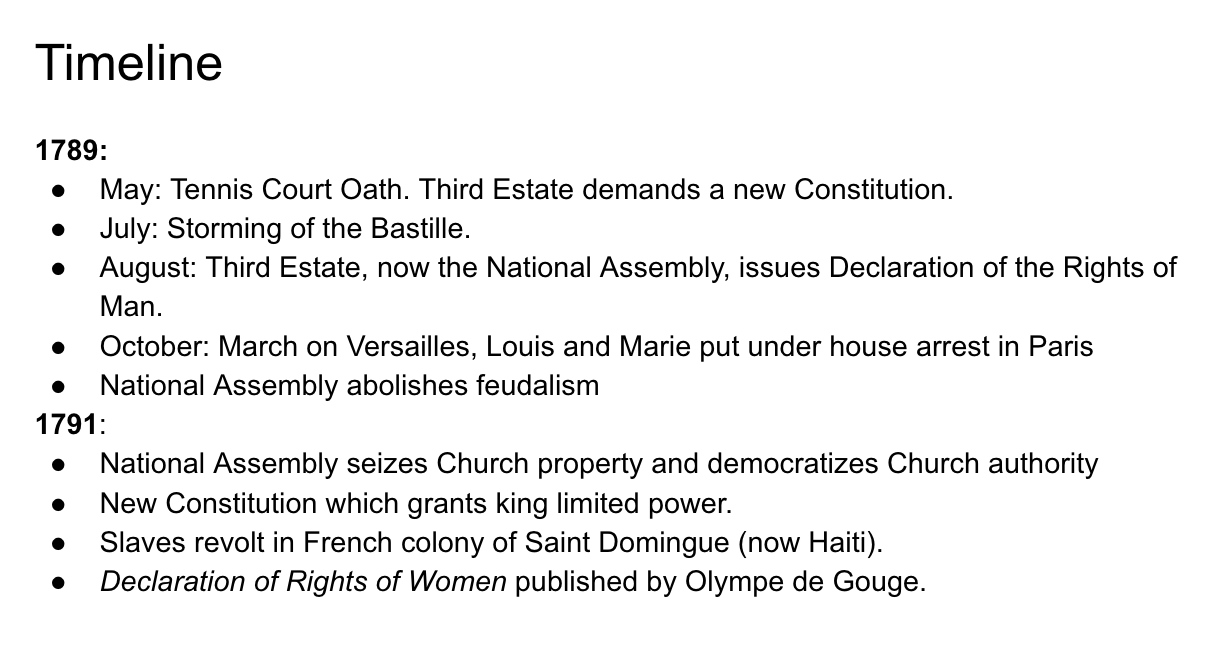
\includegraphics[width=.9\linewidth]{frenchrevtimeline.png}
\caption{French Revolution Timeline}
\end{figure}
\end{document}
